\documentclass[times, twoside]{style/axelgomez-article}
% Add "watermark" as a class option (e.g. [times, twoside, watermark]) to
% stamp every page with a "DRAFT" watermark while the article is in progress.
\usepackage{blindtext} % provides the \Blindtext / \blindtext filler text below

\usepackage{graphicx}
\graphicspath{{figures/}}

% Footer label shown next to the page numbers (e.g. journal/conference name).
\journalname{Preprint}

% Surname of the lead/corresponding author, used in the running footer.
\leadauthor{Gomez}

\begin{document}

\title{A comparative Study of Bio-Inspired Metaheuristics
  for the Estimation of Body Weight in Sheep Using Biometric Parameters}
\shorttitle{Short Running Title}

% Use letters for affiliations, numbers for equal authorship, \Letter for the corresponding author.
\author[1,\Letter]{Axel Gomez}
\author[1]{Perla Rodriguez}
\author[1]{Samuel Gualito}
\author[1]{Dario}
\author[2]{Jose Manuel Alvarez Alvarado}

\affil[1]{Universidad Autonoma de Queretaro, Department of Computer Science, Queretaro, México}
\affil[2]{Universidad Autonoma de Queretaro, Ingenieria, Queretaro, México}
\affil[3]{Third Institution, Department, City, Country}

\maketitle

%TC:break Abstract
%the command above serves to have a word count for the abstract
\begin{abstract}
\blindtext
\blindtext
\end{abstract}

%TC:break main
%the command above serves to have a word count for the abstract

\begin{keywords}
bla | bla | bla | bla
\end{keywords}

\begin{corrauthor}
axel.gomez\at example.com
\end{corrauthor}

\section*{Introduction}
\blindtext

\section*{The Body Weight Estimation Method}

\blindtext


\section*{Metaheuristic Algorithms}


  The four categories of MA are:

  \begin{itemize}
    \item Evolutionary Algorithms (EA): The theory of evolution by Darwin mentions that the 
      most fit organisms can survive and reproduce, meanwhile the less fit 
      organisms would extinct \cite{garg2010evolutionary}.
    
    \item Physical Processes (PP): The laws of physics and natural phenomena can be used as
      starting point to solve problems, where the gravity, temperature, radiation, etc. can be 
      used as inspiration to solve problems \cite{agrawal2021metaheuristic}.

    \item Swarm Intelligence (SI): It based by the nature and the behavior of the animals, 
      where it tries to mimic the the behaviour of them to achive the supervivence of the scpecies,
      by way of example, ants, wolfs, bees, birds, etc \cite{almufti2022lion}.

    \item Human Behavior (HB): The way of behave of humans across the society works as inspiration to 
      develop new MA able to solve complex problems \cite{agrawal2021metaheuristic}
        
  \end{itemize}






\subsection*{Grey Wolf Optimizer (GWO)} \blindtext

\subsection*{Cuckoo Search Algorithm (CSA)} \blindtext

\subsection*{Flying Squirrel Optimizer (FSO)} \blindtext


\subsection*{Bombardier Beetle Optimizer (BBO)} The idea is \cite{shehadeh2025bombardier} \blindtext





\section*{Results}

Just for kicks here's a citation \cite{camacho2022towards}. And a reference to a supplement \cref{note:Note1}. And \nameref{note:Note1}.
\blindtext

\begin{figure}%[tbhp]
\centering
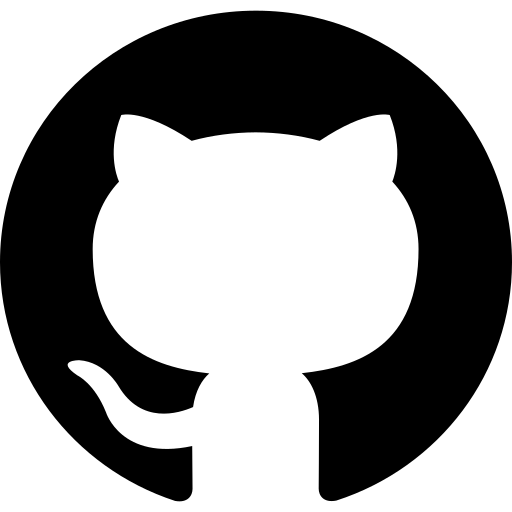
\includegraphics[width=.8\linewidth]{Figure_1}
\caption{Placeholder image with a long example caption to show justification setting.}
\label{fig:computerNo}
\end{figure}

\blindtext

Figure \ref{fig:computerNo} shows an example of how to insert a column-wide figure. To insert a figure wider than one column, please use the \verb|\begin{figure*}...\end{figure*}| environment. Figures wider than one column should be sized to 11.4 cm or 17.8 cm wide. Use \verb|\begin{SCfigure*}...\end{SCfigure*}| for a wide figure with side captions.

\vspace{1em}
\begin{table}[htp]
\begin{center}
\caption[Example results table]{Example results table, following the same layout used across my thesis chapters. Placeholder values.}
\label{tab:example}
\begin{tabular}{clclc}
\hline
Method &  & Metric &  & Value \\ \hline
\multicolumn{1}{l}{} & & \multicolumn{1}{l}{} & & \multicolumn{1}{l}{} \\

Baseline & & Accuracy & & 87.2\% \\

\multicolumn{1}{l}{} & & \multicolumn{1}{l}{} & & \multicolumn{1}{l}{} \\

Proposed & & Accuracy & & 94.6\% \\

\multicolumn{1}{l}{} & & \multicolumn{1}{l}{} & & \multicolumn{1}{l}{} \\

Proposed & & Latency (ms) & & 12.4 \\

\hline
\end{tabular}
\end{center}
\end{table}

Table \ref{tab:example} shows an example of how to insert a results table using the same style as the thesis: a centered \texttt{tabular} with horizontal rules and blank spacer rows between entries.

\section*{Discussion}

\blindtext

\section*{Conclusions}

blablaba \ref{fig:computerNo}
\blindtext

\subsection*{Future Work}
\blindtext


\section*{Bibliography}
\bibliography{bib/references}

%% You can use these special %TC: tags to ignore certain parts of the text.
%TC:ignore
%the command above ignores this section for word count
\onecolumn
\newpage

%%%%%%%%%%%%%%%%%%%%%%%%%%%%%
% Supplementary Information %
%%%%%%%%%%%%%%%%%%%%%%%%%%%%%
\captionsetup*{format=largeformat}
\section{Something about something} \label{note:Note1}
\blindtext


%TC:endignore
%the command above ignores this section for word count

\end{document}
